\section{Results and Discussion}
\label{sec:results-and-discussion}
% \subsection{Description}
% This section presents the results of your experiments,
% comparing your solution to other schemes. The metrics of
% interest are highly dependent on the topic of research, but
% should optimally cover all interesting aspects of your scheme.
% Informative graphs or tables are the key to a good result
% section.
% Furthermore, you need to discuss your results. You should
% give explanations of distinctive points and outliers in your
% results. It is also necessary to state why your scheme is
% better/worse compared to the other schemes. Thus, this section
% consists of two parts: the results of your experiments, as well
% as an explanation as to why the results are as they are

Figure \ref{fig:comparison} shows how the various prefetchers compare in terms of average speedup.
SDP, RPT and DC all perform fairly evenly.
This is to be expected, as they are all variations around the same idea.
We see that our hybrid prefetcher has lower average speedup than the simple DC implementation.
By comparing the results in greater detail, we try to understand why.

\begin{figure}
  \center
  % GNUPLOT: LaTeX picture with Postscript
\begingroup
  \makeatletter
  \providecommand\color[2][]{%
    \GenericError{(gnuplot) \space\space\space\@spaces}{%
      Package color not loaded in conjunction with
      terminal option `colourtext'%
    }{See the gnuplot documentation for explanation.%
    }{Either use 'blacktext' in gnuplot or load the package
      color.sty in LaTeX.}%
    \renewcommand\color[2][]{}%
  }%
  \providecommand\includegraphics[2][]{%
    \GenericError{(gnuplot) \space\space\space\@spaces}{%
      Package graphicx or graphics not loaded%
    }{See the gnuplot documentation for explanation.%
    }{The gnuplot epslatex terminal needs graphicx.sty or graphics.sty.}%
    \renewcommand\includegraphics[2][]{}%
  }%
  \providecommand\rotatebox[2]{#2}%
  \@ifundefined{ifGPcolor}{%
    \newif\ifGPcolor
    \GPcolorfalse
  }{}%
  \@ifundefined{ifGPblacktext}{%
    \newif\ifGPblacktext
    \GPblacktexttrue
  }{}%
  % define a \g@addto@macro without @ in the name:
  \let\gplgaddtomacro\g@addto@macro
  % define empty templates for all commands taking text:
  \gdef\gplbacktext{}%
  \gdef\gplfronttext{}%
  \makeatother
  \ifGPblacktext
    % no textcolor at all
    \def\colorrgb#1{}%
    \def\colorgray#1{}%
  \else
    % gray or color?
    \ifGPcolor
      \def\colorrgb#1{\color[rgb]{#1}}%
      \def\colorgray#1{\color[gray]{#1}}%
      \expandafter\def\csname LTw\endcsname{\color{white}}%
      \expandafter\def\csname LTb\endcsname{\color{black}}%
      \expandafter\def\csname LTa\endcsname{\color{black}}%
      \expandafter\def\csname LT0\endcsname{\color[rgb]{1,0,0}}%
      \expandafter\def\csname LT1\endcsname{\color[rgb]{0,1,0}}%
      \expandafter\def\csname LT2\endcsname{\color[rgb]{0,0,1}}%
      \expandafter\def\csname LT3\endcsname{\color[rgb]{1,0,1}}%
      \expandafter\def\csname LT4\endcsname{\color[rgb]{0,1,1}}%
      \expandafter\def\csname LT5\endcsname{\color[rgb]{1,1,0}}%
      \expandafter\def\csname LT6\endcsname{\color[rgb]{0,0,0}}%
      \expandafter\def\csname LT7\endcsname{\color[rgb]{1,0.3,0}}%
      \expandafter\def\csname LT8\endcsname{\color[rgb]{0.5,0.5,0.5}}%
    \else
      % gray
      \def\colorrgb#1{\color{black}}%
      \def\colorgray#1{\color[gray]{#1}}%
      \expandafter\def\csname LTw\endcsname{\color{white}}%
      \expandafter\def\csname LTb\endcsname{\color{black}}%
      \expandafter\def\csname LTa\endcsname{\color{black}}%
      \expandafter\def\csname LT0\endcsname{\color{black}}%
      \expandafter\def\csname LT1\endcsname{\color{black}}%
      \expandafter\def\csname LT2\endcsname{\color{black}}%
      \expandafter\def\csname LT3\endcsname{\color{black}}%
      \expandafter\def\csname LT4\endcsname{\color{black}}%
      \expandafter\def\csname LT5\endcsname{\color{black}}%
      \expandafter\def\csname LT6\endcsname{\color{black}}%
      \expandafter\def\csname LT7\endcsname{\color{black}}%
      \expandafter\def\csname LT8\endcsname{\color{black}}%
    \fi
  \fi
    \setlength{\unitlength}{0.0500bp}%
    \ifx\gptboxheight\undefined%
      \newlength{\gptboxheight}%
      \newlength{\gptboxwidth}%
      \newsavebox{\gptboxtext}%
    \fi%
    \setlength{\fboxrule}{0.5pt}%
    \setlength{\fboxsep}{1pt}%
\begin{picture}(4534.00,4534.00)%
    \gplgaddtomacro\gplbacktext{%
      \csname LTb\endcsname%
      \put(946,752){\makebox(0,0)[r]{\strut{}$1$}}%
      \put(946,1376){\makebox(0,0)[r]{\strut{}$1.02$}}%
      \put(946,2000){\makebox(0,0)[r]{\strut{}$1.04$}}%
      \put(946,2625){\makebox(0,0)[r]{\strut{}$1.06$}}%
      \put(946,3249){\makebox(0,0)[r]{\strut{}$1.08$}}%
      \put(946,3873){\makebox(0,0)[r]{\strut{}$1.1$}}%
      \put(1384,220){\makebox(0,0){\strut{}Sequential}}%
      \put(1996,220){\makebox(0,0){\strut{}SDP}}%
      \put(2608,220){\makebox(0,0){\strut{}RPT}}%
      \put(3219,220){\makebox(0,0){\strut{}DC}}%
      \put(3831,220){\makebox(0,0){\strut{}Hybrid}}%
    }%
    \gplgaddtomacro\gplfronttext{%
      \csname LTb\endcsname%
      \put(176,2156){\rotatebox{-270}{\makebox(0,0){\strut{}Average speedup}}}%
      \put(2607,4203){\makebox(0,0){\strut{}Average speedup}}%
    }%
    \gplbacktext
    \put(0,0){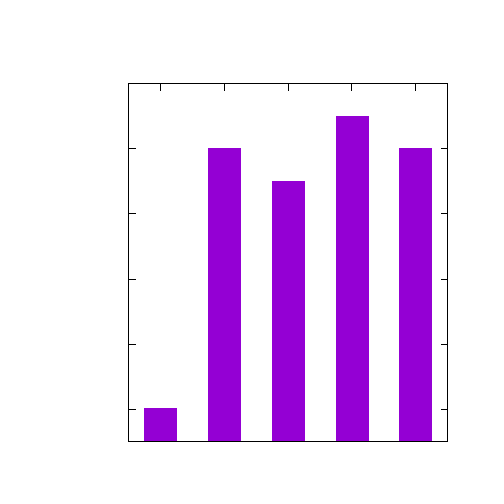
\includegraphics{plots/comparison}}%
    \gplfronttext
  \end{picture}%
\endgroup

  \caption{Average speedup for the evaluated prefetchers.}
  \label{fig:comparison}
\end{figure}



An interesting example of how the different prefetchers differ, is the \texttt{ammp} benchmark.
This is the benchmark where the sequential prefetcher performs worst;
it degrades performance significantly and a higher prefetching degree only makes
it worse.
For degree 1, it identifies just above $3.5m$ possible prefetches, but an
extremely low accuracy of only $0.1\%$ means most of the effort put into
prefetching blocks is wasted.

The SDP prefetcher on the other hand performs quite well and gives a speedup of
$1.7$ for a prefetching degree of $3$.
For this degree, the number of identified prefetches is around $8.4m$, but an
accuracy of $86\%$ means only $1.2m$ of these are wasted effort.
As the only difference between this and the sequential prefetcher is the
variable stride used for SDP, this indicates that the \texttt{ammp} benchmark
accesses memory in a linear, but strided fashion.
\todo{Is this consistent with the benchmark description?}

The remaining prefetchers all handle strided access and results comparable with
SDP should therefore be expected.
For delta correlation, the best results are achieved with a prefetching degree of $6$.
At this degree, this results in $14m$ prefetches being identified, where $84\%$
or around $12m$ turns out to be useful.
The $2.3m$ fetches for useless data is probably what makes delta correlation
less effective than SDP despite the improved coverage.
%TODO: Comment how many of these were already in MSHRs?
This is also suggested by the $44\%$ increase in average cache miss latency.

For the hybrid prefetcher developed during this project, the speedup is slightly
worse than for the pure delta correlation approach.
Despite falling back to RPT and eventually SDP, the hybrid approach identifies
fewer prefetches than the delta correlating prefetcher.
Combined with about the same accuracy as for delta correlation, this can explain
the reduced performance.
\todo{Why? It should have more}


\subsubsection{Sequential Prefetcher}
To get a sense of how the different benchmarks' performance respond to prefetching, we start by implementing a sequential prefetcher, with prefetching degree varying from 1 to 7.
The best average speedup is $1.0$ for a degree of 1.
We observe that different benchmarks respond differently to different degrees of prefetching.
See Figure \ref{fig:sequential}
\texttt{applu},


\begin{figure}
  % GNUPLOT: LaTeX picture with Postscript
\begingroup
  \makeatletter
  \providecommand\color[2][]{%
    \GenericError{(gnuplot) \space\space\space\@spaces}{%
      Package color not loaded in conjunction with
      terminal option `colourtext'%
    }{See the gnuplot documentation for explanation.%
    }{Either use 'blacktext' in gnuplot or load the package
      color.sty in LaTeX.}%
    \renewcommand\color[2][]{}%
  }%
  \providecommand\includegraphics[2][]{%
    \GenericError{(gnuplot) \space\space\space\@spaces}{%
      Package graphicx or graphics not loaded%
    }{See the gnuplot documentation for explanation.%
    }{The gnuplot epslatex terminal needs graphicx.sty or graphics.sty.}%
    \renewcommand\includegraphics[2][]{}%
  }%
  \providecommand\rotatebox[2]{#2}%
  \@ifundefined{ifGPcolor}{%
    \newif\ifGPcolor
    \GPcolorfalse
  }{}%
  \@ifundefined{ifGPblacktext}{%
    \newif\ifGPblacktext
    \GPblacktexttrue
  }{}%
  % define a \g@addto@macro without @ in the name:
  \let\gplgaddtomacro\g@addto@macro
  % define empty templates for all commands taking text:
  \gdef\gplbacktext{}%
  \gdef\gplfronttext{}%
  \makeatother
  \ifGPblacktext
    % no textcolor at all
    \def\colorrgb#1{}%
    \def\colorgray#1{}%
  \else
    % gray or color?
    \ifGPcolor
      \def\colorrgb#1{\color[rgb]{#1}}%
      \def\colorgray#1{\color[gray]{#1}}%
      \expandafter\def\csname LTw\endcsname{\color{white}}%
      \expandafter\def\csname LTb\endcsname{\color{black}}%
      \expandafter\def\csname LTa\endcsname{\color{black}}%
      \expandafter\def\csname LT0\endcsname{\color[rgb]{1,0,0}}%
      \expandafter\def\csname LT1\endcsname{\color[rgb]{0,1,0}}%
      \expandafter\def\csname LT2\endcsname{\color[rgb]{0,0,1}}%
      \expandafter\def\csname LT3\endcsname{\color[rgb]{1,0,1}}%
      \expandafter\def\csname LT4\endcsname{\color[rgb]{0,1,1}}%
      \expandafter\def\csname LT5\endcsname{\color[rgb]{1,1,0}}%
      \expandafter\def\csname LT6\endcsname{\color[rgb]{0,0,0}}%
      \expandafter\def\csname LT7\endcsname{\color[rgb]{1,0.3,0}}%
      \expandafter\def\csname LT8\endcsname{\color[rgb]{0.5,0.5,0.5}}%
    \else
      % gray
      \def\colorrgb#1{\color{black}}%
      \def\colorgray#1{\color[gray]{#1}}%
      \expandafter\def\csname LTw\endcsname{\color{white}}%
      \expandafter\def\csname LTb\endcsname{\color{black}}%
      \expandafter\def\csname LTa\endcsname{\color{black}}%
      \expandafter\def\csname LT0\endcsname{\color{black}}%
      \expandafter\def\csname LT1\endcsname{\color{black}}%
      \expandafter\def\csname LT2\endcsname{\color{black}}%
      \expandafter\def\csname LT3\endcsname{\color{black}}%
      \expandafter\def\csname LT4\endcsname{\color{black}}%
      \expandafter\def\csname LT5\endcsname{\color{black}}%
      \expandafter\def\csname LT6\endcsname{\color{black}}%
      \expandafter\def\csname LT7\endcsname{\color{black}}%
      \expandafter\def\csname LT8\endcsname{\color{black}}%
    \fi
  \fi
  \setlength{\unitlength}{0.0500bp}%
  \begin{picture}(10204.00,2834.00)%
    \gplgaddtomacro\gplbacktext{%
      \csname LTb\endcsname%
      \put(946,704){\makebox(0,0)[r]{\strut{} 0.5}}%
      \put(946,970){\makebox(0,0)[r]{\strut{} 0.6}}%
      \put(946,1237){\makebox(0,0)[r]{\strut{} 0.7}}%
      \put(946,1503){\makebox(0,0)[r]{\strut{} 0.8}}%
      \put(946,1770){\makebox(0,0)[r]{\strut{} 0.9}}%
      \put(946,2036){\makebox(0,0)[r]{\strut{} 1}}%
      \put(946,2303){\makebox(0,0)[r]{\strut{} 1.1}}%
      \put(946,2569){\makebox(0,0)[r]{\strut{} 1.2}}%
      \put(1518,484){\makebox(0,0){\strut{} 1}}%
      \put(2398,484){\makebox(0,0){\strut{} 2}}%
      \put(3277,484){\makebox(0,0){\strut{} 3}}%
      \put(4157,484){\makebox(0,0){\strut{} 4}}%
      \put(5037,484){\makebox(0,0){\strut{} 5}}%
      \put(5916,484){\makebox(0,0){\strut{} 6}}%
      \put(6796,484){\makebox(0,0){\strut{} 7}}%
      \put(176,1636){\rotatebox{-270}{\makebox(0,0){\strut{}Speedup}}}%
      \put(4157,154){\makebox(0,0){\strut{}Prefetching degree}}%
    }%
    \gplgaddtomacro\gplfronttext{%
      \csname LTb\endcsname%
      \put(9216,2459){\makebox(0,0)[r]{\strut{}ammp}}%
      \csname LTb\endcsname%
      \put(9216,2239){\makebox(0,0)[r]{\strut{}applu}}%
      \csname LTb\endcsname%
      \put(9216,2019){\makebox(0,0)[r]{\strut{}apsi}}%
      \csname LTb\endcsname%
      \put(9216,1799){\makebox(0,0)[r]{\strut{}art110}}%
      \csname LTb\endcsname%
      \put(9216,1579){\makebox(0,0)[r]{\strut{}art470}}%
      \csname LTb\endcsname%
      \put(9216,1359){\makebox(0,0)[r]{\strut{}bzip2-graphic}}%
      \csname LTb\endcsname%
      \put(9216,1139){\makebox(0,0)[r]{\strut{}bzip2-program}}%
    }%
    \gplbacktext
    \put(0,0){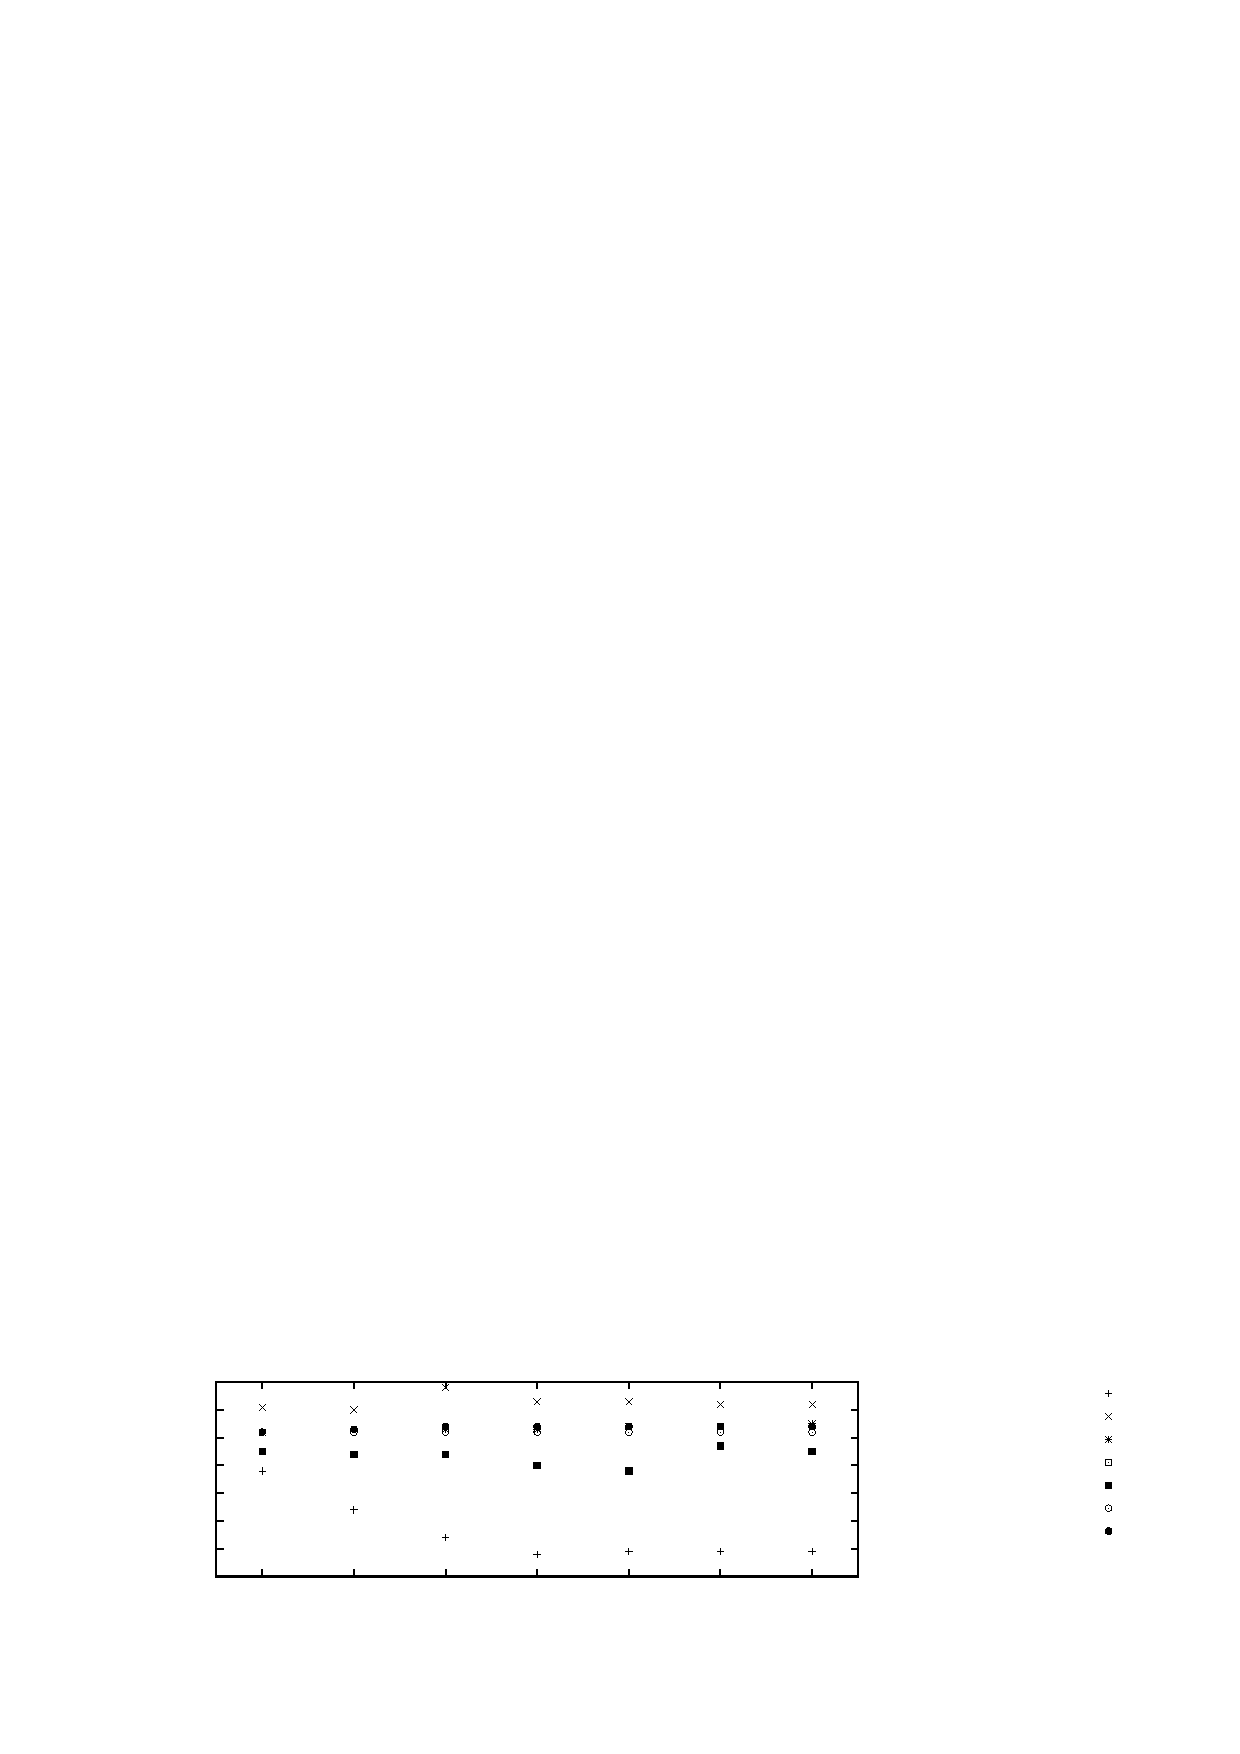
\includegraphics{plots/sequential}}%
    \gplfronttext
  \end{picture}%
\endgroup

  \caption{Effect of prefetching degree in sequential prefetcher for benchmarks.}
  \label{fig:sequential}
\end{figure}

%\begin{figure*}
%  % GNUPLOT: LaTeX picture with Postscript
\begingroup
  \makeatletter
  \providecommand\color[2][]{%
    \GenericError{(gnuplot) \space\space\space\@spaces}{%
      Package color not loaded in conjunction with
      terminal option `colourtext'%
    }{See the gnuplot documentation for explanation.%
    }{Either use 'blacktext' in gnuplot or load the package
      color.sty in LaTeX.}%
    \renewcommand\color[2][]{}%
  }%
  \providecommand\includegraphics[2][]{%
    \GenericError{(gnuplot) \space\space\space\@spaces}{%
      Package graphicx or graphics not loaded%
    }{See the gnuplot documentation for explanation.%
    }{The gnuplot epslatex terminal needs graphicx.sty or graphics.sty.}%
    \renewcommand\includegraphics[2][]{}%
  }%
  \providecommand\rotatebox[2]{#2}%
  \@ifundefined{ifGPcolor}{%
    \newif\ifGPcolor
    \GPcolorfalse
  }{}%
  \@ifundefined{ifGPblacktext}{%
    \newif\ifGPblacktext
    \GPblacktexttrue
  }{}%
  % define a \g@addto@macro without @ in the name:
  \let\gplgaddtomacro\g@addto@macro
  % define empty templates for all commands taking text:
  \gdef\gplbacktext{}%
  \gdef\gplfronttext{}%
  \makeatother
  \ifGPblacktext
    % no textcolor at all
    \def\colorrgb#1{}%
    \def\colorgray#1{}%
  \else
    % gray or color?
    \ifGPcolor
      \def\colorrgb#1{\color[rgb]{#1}}%
      \def\colorgray#1{\color[gray]{#1}}%
      \expandafter\def\csname LTw\endcsname{\color{white}}%
      \expandafter\def\csname LTb\endcsname{\color{black}}%
      \expandafter\def\csname LTa\endcsname{\color{black}}%
      \expandafter\def\csname LT0\endcsname{\color[rgb]{1,0,0}}%
      \expandafter\def\csname LT1\endcsname{\color[rgb]{0,1,0}}%
      \expandafter\def\csname LT2\endcsname{\color[rgb]{0,0,1}}%
      \expandafter\def\csname LT3\endcsname{\color[rgb]{1,0,1}}%
      \expandafter\def\csname LT4\endcsname{\color[rgb]{0,1,1}}%
      \expandafter\def\csname LT5\endcsname{\color[rgb]{1,1,0}}%
      \expandafter\def\csname LT6\endcsname{\color[rgb]{0,0,0}}%
      \expandafter\def\csname LT7\endcsname{\color[rgb]{1,0.3,0}}%
      \expandafter\def\csname LT8\endcsname{\color[rgb]{0.5,0.5,0.5}}%
    \else
      % gray
      \def\colorrgb#1{\color{black}}%
      \def\colorgray#1{\color[gray]{#1}}%
      \expandafter\def\csname LTw\endcsname{\color{white}}%
      \expandafter\def\csname LTb\endcsname{\color{black}}%
      \expandafter\def\csname LTa\endcsname{\color{black}}%
      \expandafter\def\csname LT0\endcsname{\color{black}}%
      \expandafter\def\csname LT1\endcsname{\color{black}}%
      \expandafter\def\csname LT2\endcsname{\color{black}}%
      \expandafter\def\csname LT3\endcsname{\color{black}}%
      \expandafter\def\csname LT4\endcsname{\color{black}}%
      \expandafter\def\csname LT5\endcsname{\color{black}}%
      \expandafter\def\csname LT6\endcsname{\color{black}}%
      \expandafter\def\csname LT7\endcsname{\color{black}}%
      \expandafter\def\csname LT8\endcsname{\color{black}}%
    \fi
  \fi
    \setlength{\unitlength}{0.0500bp}%
    \ifx\gptboxheight\undefined%
      \newlength{\gptboxheight}%
      \newlength{\gptboxwidth}%
      \newsavebox{\gptboxtext}%
    \fi%
    \setlength{\fboxrule}{0.5pt}%
    \setlength{\fboxsep}{1pt}%
\begin{picture}(7200.00,5040.00)%
    \gplgaddtomacro\gplbacktext{%
      \csname LTb\endcsname%
      \put(814,2263){\makebox(0,0)[r]{\strut{}$0.5$}}%
      \put(814,2545){\makebox(0,0)[r]{\strut{}$0.6$}}%
      \put(814,2827){\makebox(0,0)[r]{\strut{}$0.7$}}%
      \put(814,3109){\makebox(0,0)[r]{\strut{}$0.8$}}%
      \put(814,3392){\makebox(0,0)[r]{\strut{}$0.9$}}%
      \put(814,3674){\makebox(0,0)[r]{\strut{}$1$}}%
      \put(814,3956){\makebox(0,0)[r]{\strut{}$1.1$}}%
      \put(814,4238){\makebox(0,0)[r]{\strut{}$1.2$}}%
      \put(1190,2068){\rotatebox{-270}{\makebox(0,0)[r]{\strut{}ammp}}}%
      \put(1678,2068){\rotatebox{-270}{\makebox(0,0)[r]{\strut{}art110}}}%
      \put(2166,2068){\rotatebox{-270}{\makebox(0,0)[r]{\strut{}art470}}}%
      \put(2654,2068){\rotatebox{-270}{\makebox(0,0)[r]{\strut{}twolf}}}%
      \put(3142,2068){\rotatebox{-270}{\makebox(0,0)[r]{\strut{}swim}}}%
      \put(3630,2068){\rotatebox{-270}{\makebox(0,0)[r]{\strut{}bzip2-source}}}%
      \put(4119,2068){\rotatebox{-270}{\makebox(0,0)[r]{\strut{}bzip2-graphic}}}%
      \put(4607,2068){\rotatebox{-270}{\makebox(0,0)[r]{\strut{}apsi}}}%
      \put(5095,2068){\rotatebox{-270}{\makebox(0,0)[r]{\strut{}bzip2-program}}}%
      \put(5583,2068){\rotatebox{-270}{\makebox(0,0)[r]{\strut{}galgel}}}%
      \put(6071,2068){\rotatebox{-270}{\makebox(0,0)[r]{\strut{}applu}}}%
      \put(6559,2068){\rotatebox{-270}{\makebox(0,0)[r]{\strut{}wupwise}}}%
    }%
    \gplgaddtomacro\gplfronttext{%
      \csname LTb\endcsname%
      \put(176,3321){\rotatebox{-270}{\makebox(0,0){\strut{}Speedup}}}%
      \put(3874,154){\makebox(0,0){\strut{}Benchmark}}%
      \put(3874,4709){\makebox(0,0){\strut{}Sequential prefetcher (p=3) performance}}%
    }%
    \gplbacktext
    \put(0,0){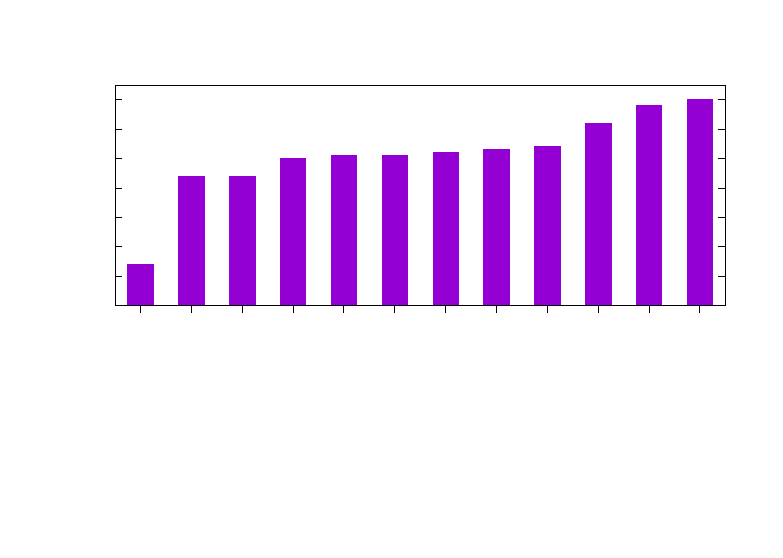
\includegraphics{plots/seq3}}%
    \gplfronttext
  \end{picture}%
\endgroup

%  \caption{Performance of sequential prefetcher with $p = 3$ across benchmarks.}
%  \label{fig:seq3}
%\end{figure*}

\subsubsection{Stride Direct Prefetcher}
A simple implementation of a stride direct prefetcher yielded a better average speedup ($1.07$) than the sequential prefetcher.
The benchmarks wupwise and ammp had high speedups, which pulled up the average.
This prefetcher had a negative impact on the twolf benchmark.


\subsubsection{Reference Prediction Table}
// TODO: 
The RPT implementation yielded an average speedup of $1.06$.
While slightly lower than the SDP average, the maximum and minimum values are closer together.
Testing of the RPT implementation saw no benchmark with a speedup of less than $0.95$.
Figure~\ref{fig:rpt} shows how RPT performs on each benchmark.

%\begin{figure*}
%  % GNUPLOT: LaTeX picture with Postscript
\begingroup
  \makeatletter
  \providecommand\color[2][]{%
    \GenericError{(gnuplot) \space\space\space\@spaces}{%
      Package color not loaded in conjunction with
      terminal option `colourtext'%
    }{See the gnuplot documentation for explanation.%
    }{Either use 'blacktext' in gnuplot or load the package
      color.sty in LaTeX.}%
    \renewcommand\color[2][]{}%
  }%
  \providecommand\includegraphics[2][]{%
    \GenericError{(gnuplot) \space\space\space\@spaces}{%
      Package graphicx or graphics not loaded%
    }{See the gnuplot documentation for explanation.%
    }{The gnuplot epslatex terminal needs graphicx.sty or graphics.sty.}%
    \renewcommand\includegraphics[2][]{}%
  }%
  \providecommand\rotatebox[2]{#2}%
  \@ifundefined{ifGPcolor}{%
    \newif\ifGPcolor
    \GPcolorfalse
  }{}%
  \@ifundefined{ifGPblacktext}{%
    \newif\ifGPblacktext
    \GPblacktexttrue
  }{}%
  % define a \g@addto@macro without @ in the name:
  \let\gplgaddtomacro\g@addto@macro
  % define empty templates for all commands taking text:
  \gdef\gplbacktext{}%
  \gdef\gplfronttext{}%
  \makeatother
  \ifGPblacktext
    % no textcolor at all
    \def\colorrgb#1{}%
    \def\colorgray#1{}%
  \else
    % gray or color?
    \ifGPcolor
      \def\colorrgb#1{\color[rgb]{#1}}%
      \def\colorgray#1{\color[gray]{#1}}%
      \expandafter\def\csname LTw\endcsname{\color{white}}%
      \expandafter\def\csname LTb\endcsname{\color{black}}%
      \expandafter\def\csname LTa\endcsname{\color{black}}%
      \expandafter\def\csname LT0\endcsname{\color[rgb]{1,0,0}}%
      \expandafter\def\csname LT1\endcsname{\color[rgb]{0,1,0}}%
      \expandafter\def\csname LT2\endcsname{\color[rgb]{0,0,1}}%
      \expandafter\def\csname LT3\endcsname{\color[rgb]{1,0,1}}%
      \expandafter\def\csname LT4\endcsname{\color[rgb]{0,1,1}}%
      \expandafter\def\csname LT5\endcsname{\color[rgb]{1,1,0}}%
      \expandafter\def\csname LT6\endcsname{\color[rgb]{0,0,0}}%
      \expandafter\def\csname LT7\endcsname{\color[rgb]{1,0.3,0}}%
      \expandafter\def\csname LT8\endcsname{\color[rgb]{0.5,0.5,0.5}}%
    \else
      % gray
      \def\colorrgb#1{\color{black}}%
      \def\colorgray#1{\color[gray]{#1}}%
      \expandafter\def\csname LTw\endcsname{\color{white}}%
      \expandafter\def\csname LTb\endcsname{\color{black}}%
      \expandafter\def\csname LTa\endcsname{\color{black}}%
      \expandafter\def\csname LT0\endcsname{\color{black}}%
      \expandafter\def\csname LT1\endcsname{\color{black}}%
      \expandafter\def\csname LT2\endcsname{\color{black}}%
      \expandafter\def\csname LT3\endcsname{\color{black}}%
      \expandafter\def\csname LT4\endcsname{\color{black}}%
      \expandafter\def\csname LT5\endcsname{\color{black}}%
      \expandafter\def\csname LT6\endcsname{\color{black}}%
      \expandafter\def\csname LT7\endcsname{\color{black}}%
      \expandafter\def\csname LT8\endcsname{\color{black}}%
    \fi
  \fi
    \setlength{\unitlength}{0.0500bp}%
    \ifx\gptboxheight\undefined%
      \newlength{\gptboxheight}%
      \newlength{\gptboxwidth}%
      \newsavebox{\gptboxtext}%
    \fi%
    \setlength{\fboxrule}{0.5pt}%
    \setlength{\fboxsep}{1pt}%
\begin{picture}(7200.00,5040.00)%
    \gplgaddtomacro\gplbacktext{%
      \csname LTb\endcsname%
      \put(814,2263){\makebox(0,0)[r]{\strut{}$0.5$}}%
      \put(814,2545){\makebox(0,0)[r]{\strut{}$0.6$}}%
      \put(814,2827){\makebox(0,0)[r]{\strut{}$0.7$}}%
      \put(814,3109){\makebox(0,0)[r]{\strut{}$0.8$}}%
      \put(814,3392){\makebox(0,0)[r]{\strut{}$0.9$}}%
      \put(814,3674){\makebox(0,0)[r]{\strut{}$1$}}%
      \put(814,3956){\makebox(0,0)[r]{\strut{}$1.1$}}%
      \put(814,4238){\makebox(0,0)[r]{\strut{}$1.2$}}%
      \put(1190,2068){\rotatebox{-270}{\makebox(0,0)[r]{\strut{}bzip2-source}}}%
      \put(1678,2068){\rotatebox{-270}{\makebox(0,0)[r]{\strut{}twolf}}}%
      \put(2166,2068){\rotatebox{-270}{\makebox(0,0)[r]{\strut{}swim}}}%
      \put(2654,2068){\rotatebox{-270}{\makebox(0,0)[r]{\strut{}apsi}}}%
      \put(3142,2068){\rotatebox{-270}{\makebox(0,0)[r]{\strut{}galgel}}}%
      \put(3630,2068){\rotatebox{-270}{\makebox(0,0)[r]{\strut{}bzip2-graphic}}}%
      \put(4119,2068){\rotatebox{-270}{\makebox(0,0)[r]{\strut{}art110}}}%
      \put(4607,2068){\rotatebox{-270}{\makebox(0,0)[r]{\strut{}art470}}}%
      \put(5095,2068){\rotatebox{-270}{\makebox(0,0)[r]{\strut{}bzip2-program}}}%
      \put(5583,2068){\rotatebox{-270}{\makebox(0,0)[r]{\strut{}applu}}}%
      \put(6071,2068){\rotatebox{-270}{\makebox(0,0)[r]{\strut{}wupwise}}}%
      \put(6559,2068){\rotatebox{-270}{\makebox(0,0)[r]{\strut{}ammp}}}%
    }%
    \gplgaddtomacro\gplfronttext{%
      \csname LTb\endcsname%
      \put(176,3321){\rotatebox{-270}{\makebox(0,0){\strut{}Speedup}}}%
      \put(3874,154){\makebox(0,0){\strut{}Benchmark}}%
      \put(3874,4709){\makebox(0,0){\strut{}Reference Prediction Table}}%
    }%
    \gplbacktext
    \put(0,0){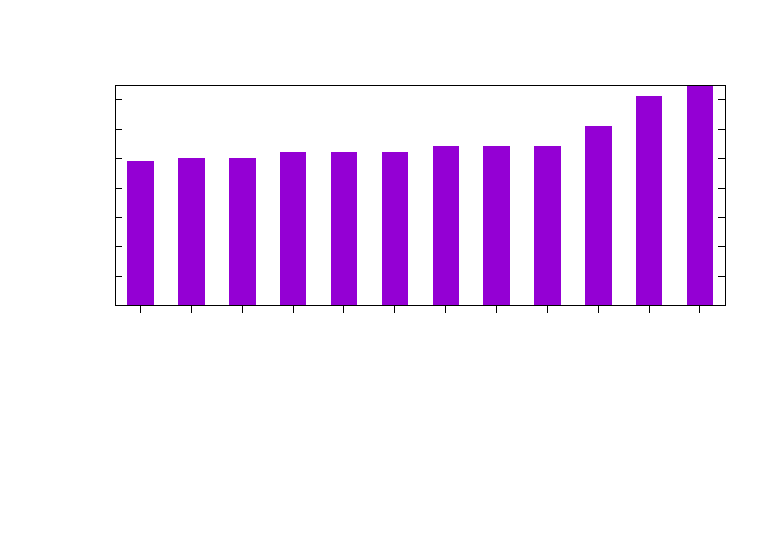
\includegraphics{plots/rpt}}%
    \gplfronttext
  \end{picture}%
\endgroup

%  \caption{Performance of RPT prefetcher across benchmarks.}
%  \label{fig:rpt}
%\end{figure*}

\subsubsection{Global History Buffer with Delta Correlation}
The implementation of the global history buffer with SDP and RTP as fallback was successfully implemented and yielded the speedups shown in Figure \ref{fig:ghbdc}.
The best speedup was acquired for the ammp benchmark, but many of the other benchmark showed only a slight speedup if any at all.


\begin{figure*}
  % GNUPLOT: LaTeX picture with Postscript
\begingroup
  \makeatletter
  \providecommand\color[2][]{%
    \GenericError{(gnuplot) \space\space\space\@spaces}{%
      Package color not loaded in conjunction with
      terminal option `colourtext'%
    }{See the gnuplot documentation for explanation.%
    }{Either use 'blacktext' in gnuplot or load the package
      color.sty in LaTeX.}%
    \renewcommand\color[2][]{}%
  }%
  \providecommand\includegraphics[2][]{%
    \GenericError{(gnuplot) \space\space\space\@spaces}{%
      Package graphicx or graphics not loaded%
    }{See the gnuplot documentation for explanation.%
    }{The gnuplot epslatex terminal needs graphicx.sty or graphics.sty.}%
    \renewcommand\includegraphics[2][]{}%
  }%
  \providecommand\rotatebox[2]{#2}%
  \@ifundefined{ifGPcolor}{%
    \newif\ifGPcolor
    \GPcolorfalse
  }{}%
  \@ifundefined{ifGPblacktext}{%
    \newif\ifGPblacktext
    \GPblacktexttrue
  }{}%
  % define a \g@addto@macro without @ in the name:
  \let\gplgaddtomacro\g@addto@macro
  % define empty templates for all commands taking text:
  \gdef\gplbacktext{}%
  \gdef\gplfronttext{}%
  \makeatother
  \ifGPblacktext
    % no textcolor at all
    \def\colorrgb#1{}%
    \def\colorgray#1{}%
  \else
    % gray or color?
    \ifGPcolor
      \def\colorrgb#1{\color[rgb]{#1}}%
      \def\colorgray#1{\color[gray]{#1}}%
      \expandafter\def\csname LTw\endcsname{\color{white}}%
      \expandafter\def\csname LTb\endcsname{\color{black}}%
      \expandafter\def\csname LTa\endcsname{\color{black}}%
      \expandafter\def\csname LT0\endcsname{\color[rgb]{1,0,0}}%
      \expandafter\def\csname LT1\endcsname{\color[rgb]{0,1,0}}%
      \expandafter\def\csname LT2\endcsname{\color[rgb]{0,0,1}}%
      \expandafter\def\csname LT3\endcsname{\color[rgb]{1,0,1}}%
      \expandafter\def\csname LT4\endcsname{\color[rgb]{0,1,1}}%
      \expandafter\def\csname LT5\endcsname{\color[rgb]{1,1,0}}%
      \expandafter\def\csname LT6\endcsname{\color[rgb]{0,0,0}}%
      \expandafter\def\csname LT7\endcsname{\color[rgb]{1,0.3,0}}%
      \expandafter\def\csname LT8\endcsname{\color[rgb]{0.5,0.5,0.5}}%
    \else
      % gray
      \def\colorrgb#1{\color{black}}%
      \def\colorgray#1{\color[gray]{#1}}%
      \expandafter\def\csname LTw\endcsname{\color{white}}%
      \expandafter\def\csname LTb\endcsname{\color{black}}%
      \expandafter\def\csname LTa\endcsname{\color{black}}%
      \expandafter\def\csname LT0\endcsname{\color{black}}%
      \expandafter\def\csname LT1\endcsname{\color{black}}%
      \expandafter\def\csname LT2\endcsname{\color{black}}%
      \expandafter\def\csname LT3\endcsname{\color{black}}%
      \expandafter\def\csname LT4\endcsname{\color{black}}%
      \expandafter\def\csname LT5\endcsname{\color{black}}%
      \expandafter\def\csname LT6\endcsname{\color{black}}%
      \expandafter\def\csname LT7\endcsname{\color{black}}%
      \expandafter\def\csname LT8\endcsname{\color{black}}%
    \fi
  \fi
  \setlength{\unitlength}{0.0500bp}%
  \begin{picture}(10204.00,2834.00)%
    \gplgaddtomacro\gplbacktext{%
      \csname LTb\endcsname%
      \put(946,704){\makebox(0,0)[r]{\strut{} 1}}%
      \put(946,970){\makebox(0,0)[r]{\strut{} 1.1}}%
      \put(946,1237){\makebox(0,0)[r]{\strut{} 1.2}}%
      \put(946,1503){\makebox(0,0)[r]{\strut{} 1.3}}%
      \put(946,1770){\makebox(0,0)[r]{\strut{} 1.4}}%
      \put(946,2036){\makebox(0,0)[r]{\strut{} 1.5}}%
      \put(946,2303){\makebox(0,0)[r]{\strut{} 1.6}}%
      \put(946,2569){\makebox(0,0)[r]{\strut{} 1.7}}%
      \put(1518,484){\makebox(0,0){\strut{} 1}}%
      \put(2398,484){\makebox(0,0){\strut{} 2}}%
      \put(3277,484){\makebox(0,0){\strut{} 3}}%
      \put(4157,484){\makebox(0,0){\strut{} 4}}%
      \put(5037,484){\makebox(0,0){\strut{} 5}}%
      \put(5916,484){\makebox(0,0){\strut{} 6}}%
      \put(6796,484){\makebox(0,0){\strut{} 7}}%
      \put(176,1636){\rotatebox{-270}{\makebox(0,0){\strut{}Speedup}}}%
      \put(4157,154){\makebox(0,0){\strut{}Prefetching degree}}%
    }%
    \gplgaddtomacro\gplfronttext{%
      \csname LTb\endcsname%
      \put(9216,2459){\makebox(0,0)[r]{\strut{}ammp}}%
      \csname LTb\endcsname%
      \put(9216,2239){\makebox(0,0)[r]{\strut{}applu}}%
      \csname LTb\endcsname%
      \put(9216,2019){\makebox(0,0)[r]{\strut{}apsi}}%
      \csname LTb\endcsname%
      \put(9216,1799){\makebox(0,0)[r]{\strut{}art110}}%
      \csname LTb\endcsname%
      \put(9216,1579){\makebox(0,0)[r]{\strut{}art470}}%
      \csname LTb\endcsname%
      \put(9216,1359){\makebox(0,0)[r]{\strut{}bzip2-graphic}}%
      \csname LTb\endcsname%
      \put(9216,1139){\makebox(0,0)[r]{\strut{}bzip2-program}}%
    }%
    \gplbacktext
    \put(0,0){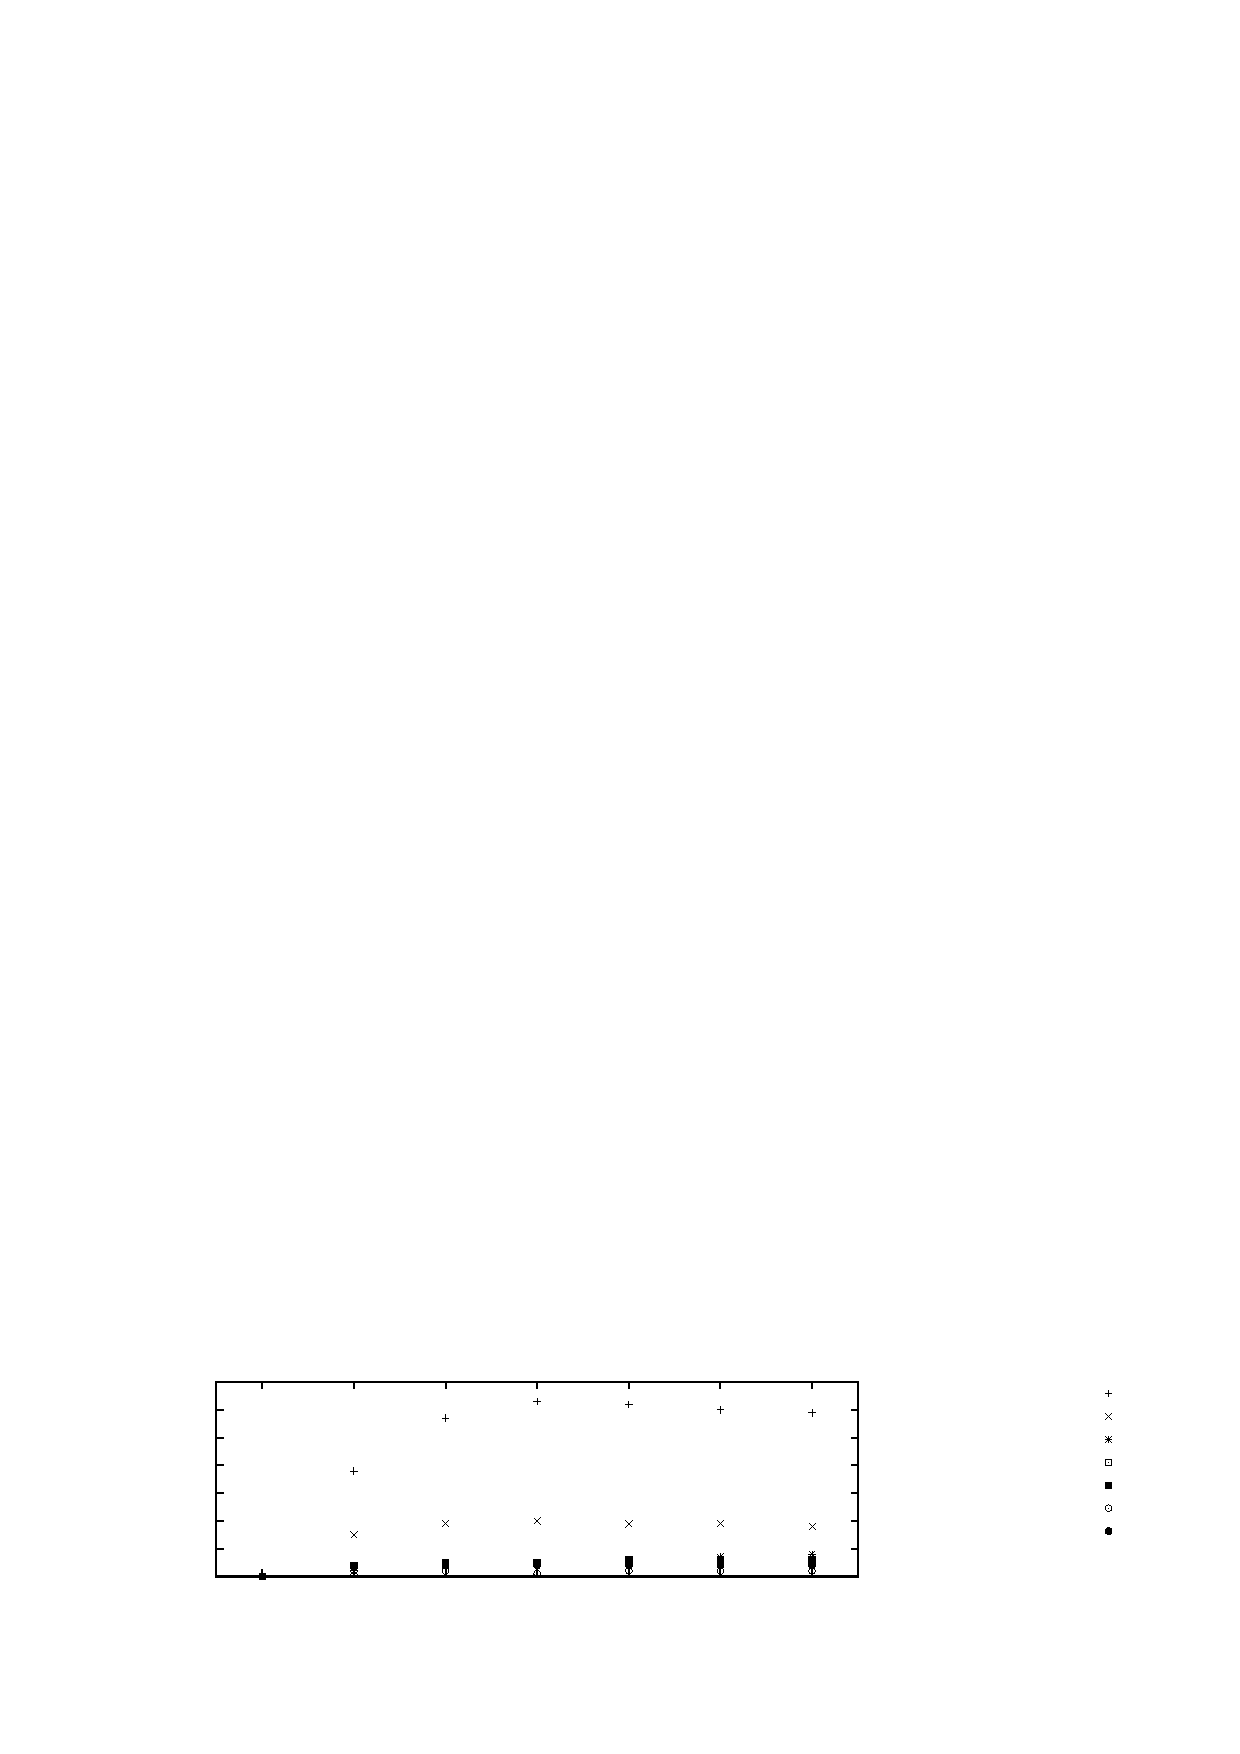
\includegraphics{plots/ghbdc}}%
    \gplfronttext
  \end{picture}%
\endgroup

  \caption{Speedup of each benchmark as a function of degree for the global history buffer with delta correlation and fall back to SDP and RTP.}
  \label{fig:ghbdc}
\end{figure*}

\begin{figure*}
  % GNUPLOT: LaTeX picture with Postscript
\begingroup
  \makeatletter
  \providecommand\color[2][]{%
    \GenericError{(gnuplot) \space\space\space\@spaces}{%
      Package color not loaded in conjunction with
      terminal option `colourtext'%
    }{See the gnuplot documentation for explanation.%
    }{Either use 'blacktext' in gnuplot or load the package
      color.sty in LaTeX.}%
    \renewcommand\color[2][]{}%
  }%
  \providecommand\includegraphics[2][]{%
    \GenericError{(gnuplot) \space\space\space\@spaces}{%
      Package graphicx or graphics not loaded%
    }{See the gnuplot documentation for explanation.%
    }{The gnuplot epslatex terminal needs graphicx.sty or graphics.sty.}%
    \renewcommand\includegraphics[2][]{}%
  }%
  \providecommand\rotatebox[2]{#2}%
  \@ifundefined{ifGPcolor}{%
    \newif\ifGPcolor
    \GPcolorfalse
  }{}%
  \@ifundefined{ifGPblacktext}{%
    \newif\ifGPblacktext
    \GPblacktexttrue
  }{}%
  % define a \g@addto@macro without @ in the name:
  \let\gplgaddtomacro\g@addto@macro
  % define empty templates for all commands taking text:
  \gdef\gplbacktext{}%
  \gdef\gplfronttext{}%
  \makeatother
  \ifGPblacktext
    % no textcolor at all
    \def\colorrgb#1{}%
    \def\colorgray#1{}%
  \else
    % gray or color?
    \ifGPcolor
      \def\colorrgb#1{\color[rgb]{#1}}%
      \def\colorgray#1{\color[gray]{#1}}%
      \expandafter\def\csname LTw\endcsname{\color{white}}%
      \expandafter\def\csname LTb\endcsname{\color{black}}%
      \expandafter\def\csname LTa\endcsname{\color{black}}%
      \expandafter\def\csname LT0\endcsname{\color[rgb]{1,0,0}}%
      \expandafter\def\csname LT1\endcsname{\color[rgb]{0,1,0}}%
      \expandafter\def\csname LT2\endcsname{\color[rgb]{0,0,1}}%
      \expandafter\def\csname LT3\endcsname{\color[rgb]{1,0,1}}%
      \expandafter\def\csname LT4\endcsname{\color[rgb]{0,1,1}}%
      \expandafter\def\csname LT5\endcsname{\color[rgb]{1,1,0}}%
      \expandafter\def\csname LT6\endcsname{\color[rgb]{0,0,0}}%
      \expandafter\def\csname LT7\endcsname{\color[rgb]{1,0.3,0}}%
      \expandafter\def\csname LT8\endcsname{\color[rgb]{0.5,0.5,0.5}}%
    \else
      % gray
      \def\colorrgb#1{\color{black}}%
      \def\colorgray#1{\color[gray]{#1}}%
      \expandafter\def\csname LTw\endcsname{\color{white}}%
      \expandafter\def\csname LTb\endcsname{\color{black}}%
      \expandafter\def\csname LTa\endcsname{\color{black}}%
      \expandafter\def\csname LT0\endcsname{\color{black}}%
      \expandafter\def\csname LT1\endcsname{\color{black}}%
      \expandafter\def\csname LT2\endcsname{\color{black}}%
      \expandafter\def\csname LT3\endcsname{\color{black}}%
      \expandafter\def\csname LT4\endcsname{\color{black}}%
      \expandafter\def\csname LT5\endcsname{\color{black}}%
      \expandafter\def\csname LT6\endcsname{\color{black}}%
      \expandafter\def\csname LT7\endcsname{\color{black}}%
      \expandafter\def\csname LT8\endcsname{\color{black}}%
    \fi
  \fi
    \setlength{\unitlength}{0.0500bp}%
    \ifx\gptboxheight\undefined%
      \newlength{\gptboxheight}%
      \newlength{\gptboxwidth}%
      \newsavebox{\gptboxtext}%
    \fi%
    \setlength{\fboxrule}{0.5pt}%
    \setlength{\fboxsep}{1pt}%
\begin{picture}(7200.00,5040.00)%
    \gplgaddtomacro\gplbacktext{%
      \csname LTb\endcsname%
      \put(946,949){\makebox(0,0)[r]{\strut{}$0.96$}}%
      \put(946,1439){\makebox(0,0)[r]{\strut{}$0.98$}}%
      \put(946,1929){\makebox(0,0)[r]{\strut{}$1$}}%
      \put(946,2419){\makebox(0,0)[r]{\strut{}$1.02$}}%
      \put(946,2909){\makebox(0,0)[r]{\strut{}$1.04$}}%
      \put(946,3399){\makebox(0,0)[r]{\strut{}$1.06$}}%
      \put(946,3889){\makebox(0,0)[r]{\strut{}$1.08$}}%
      \put(946,4379){\makebox(0,0)[r]{\strut{}$1.1$}}%
      \put(1487,484){\makebox(0,0){\strut{}1}}%
      \put(2305,484){\makebox(0,0){\strut{}2}}%
      \put(3123,484){\makebox(0,0){\strut{}3}}%
      \put(3941,484){\makebox(0,0){\strut{}4}}%
      \put(4758,484){\makebox(0,0){\strut{}5}}%
      \put(5576,484){\makebox(0,0){\strut{}6}}%
      \put(6394,484){\makebox(0,0){\strut{}7}}%
    }%
    \gplgaddtomacro\gplfronttext{%
      \csname LTb\endcsname%
      \put(176,2541){\rotatebox{-270}{\makebox(0,0){\strut{}Average speedup}}}%
      \put(3940,154){\makebox(0,0){\strut{}Prefetching degree}}%
      \put(3940,4709){\makebox(0,0){\strut{}Performance of GHB-based DC/RPT/SDP hybrid prefetcher}}%
    }%
    \gplbacktext
    \put(0,0){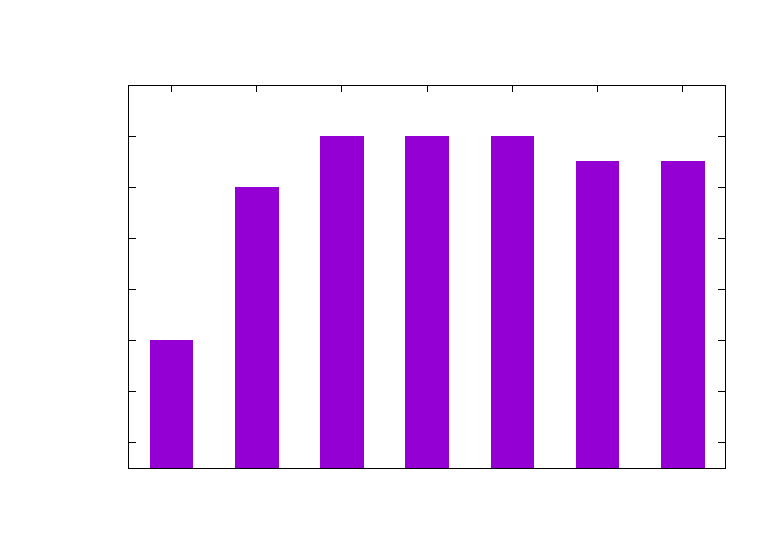
\includegraphics{plots/ghbdcavg}}%
    \gplfronttext
  \end{picture}%
\endgroup

  \caption{Average speedup as a function of prefetching degree for our final prefetcher implementation.}
  \label{fig:ghbdcavg}
\end{figure*}

%\subsection{Description}
% This section might elaborate on alternative approaches that
% you have tried, but were not successful. It discusses weaknesses
% of your scheme and highlights the strong and weak
% points of your experimental setup.

Experimenting with sequential prefetching of various degrees yielded surprisingly good results for some benchmarks.
A possible explanation for this is that the benchmark's behavior matched exceptionally well with the assumptions used when creating the prefetcher.
Based on this, it is reasonable to assume that the \texttt{applu} and \texttt{wupwise} benchmarks access memory fairly sequentially.

\todo{SDP}
\todo{RPT}

Our hybrid implementation
More interesting to note, is that the delta-correlation implementation does an exceptionally good job at the \texttt{ammp} benchmark.
This was the benchmark with the highest negative performance impact from the naive sequential prefetcher, but the memory pattern seems to be very well suited for delta correlation.
